



\subsection{The L=2 case}

As the Monte Carlo cycles increases, the mean energy in figure \ref{fig:l2energy} stabilizes around the analytical value for $ T = 1 \frac{k_BT}{J}$, which is calculated from equation \ref{eq:L2_E}. After it reaches equilibrium around $0.25\E{7} $ MC cycles, it is however not constant and fluctuates. In addition it is not aligning perfectly with the analytical value, but it is accurate to the fourth digit. This can be seen from figure \ref{fig:abserror}. 

Figure \ref{fig:l2magmagabs} shows the same trend for $ \langle \abs{M} \rangle $ and $ \langle {M} \rangle $. Both measurements equilibrates in roughly the same amount of MC-cycles, but there is a significant difference in the behaviour after  equilibrium is reached. $ \langle {M} \rangle $ is fluctuating much more about the analytical value. All calculations in this subsection are at T = 1.0 $ \frac{k_BT	}{J} $. 



	\begin{figure}[H]
	\begin{subfigure}[b]{0.49\textwidth}
	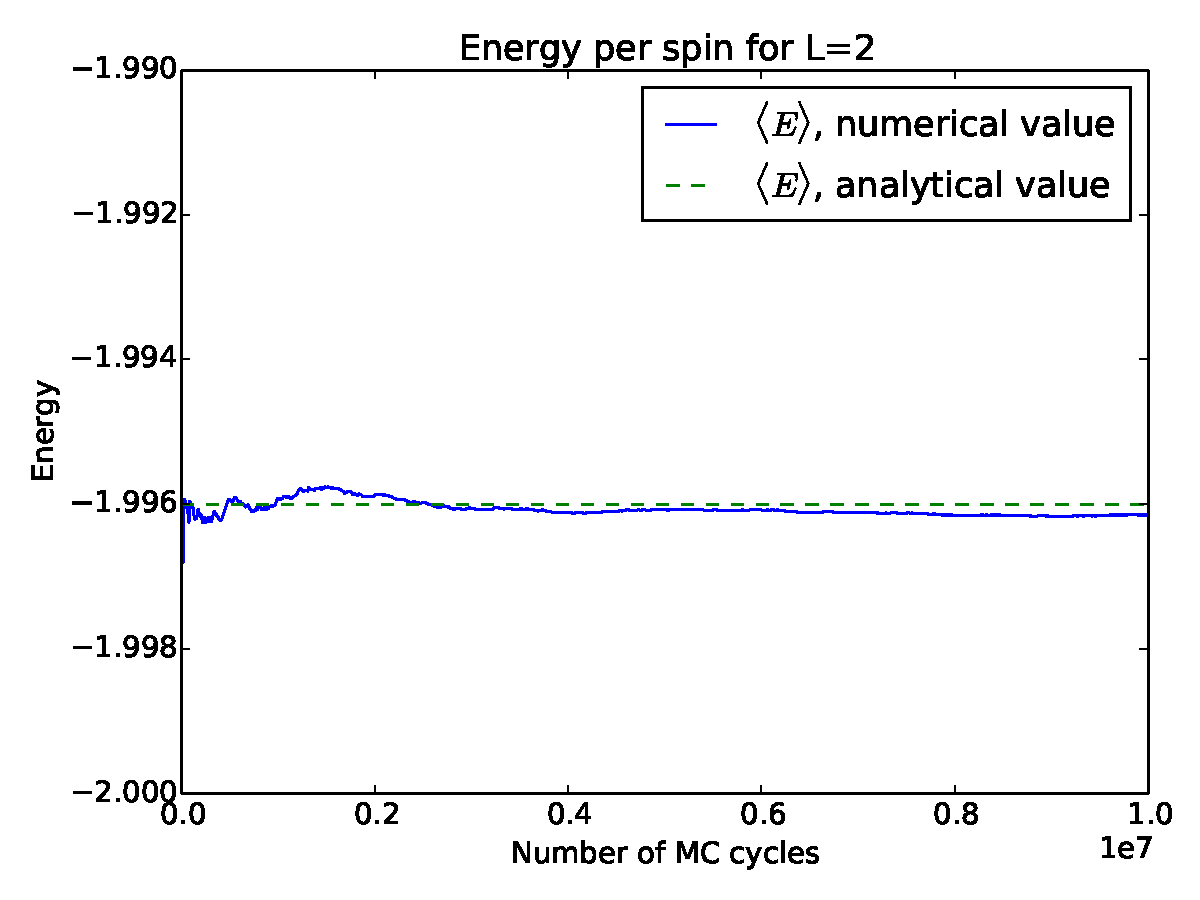
\includegraphics[width=1\linewidth]{../results/4b/L_2_energy}
\caption{Mean energy as a function of Monte Carlo cycles. }
\label{fig:l2energy}
	\end{subfigure}
	\hfill
	\begin{subfigure}[b]{0.49\textwidth}
	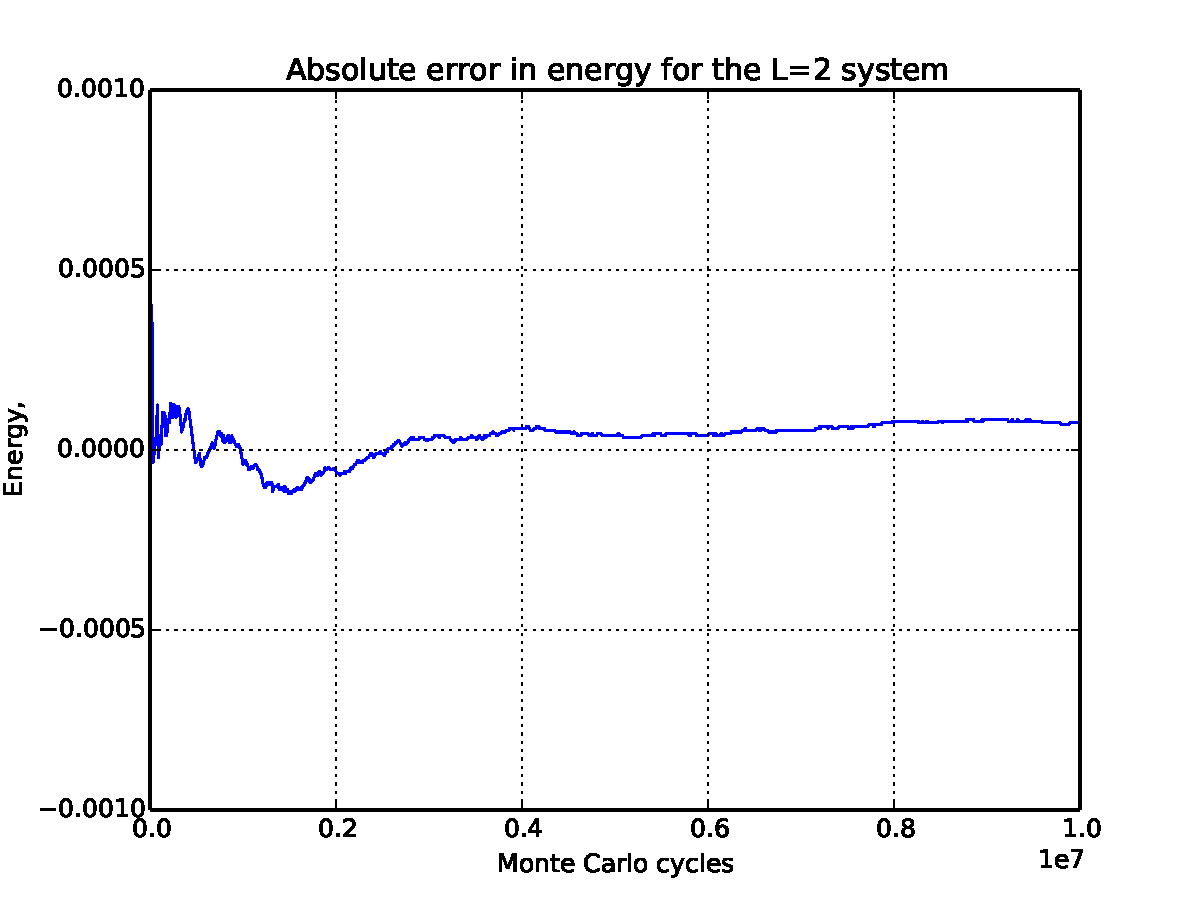
\includegraphics[width=1\linewidth]{../results/4b/abs_error}
\caption{Mean absolute error for the energy}
\label{fig:abserror}
	\end{subfigure}
	\caption{Mean energy and mean absolute error of the energy at $T=1 \frac{k_BT}{J}$.}
\end{figure}

\begin{figure}[H]
	\centering
	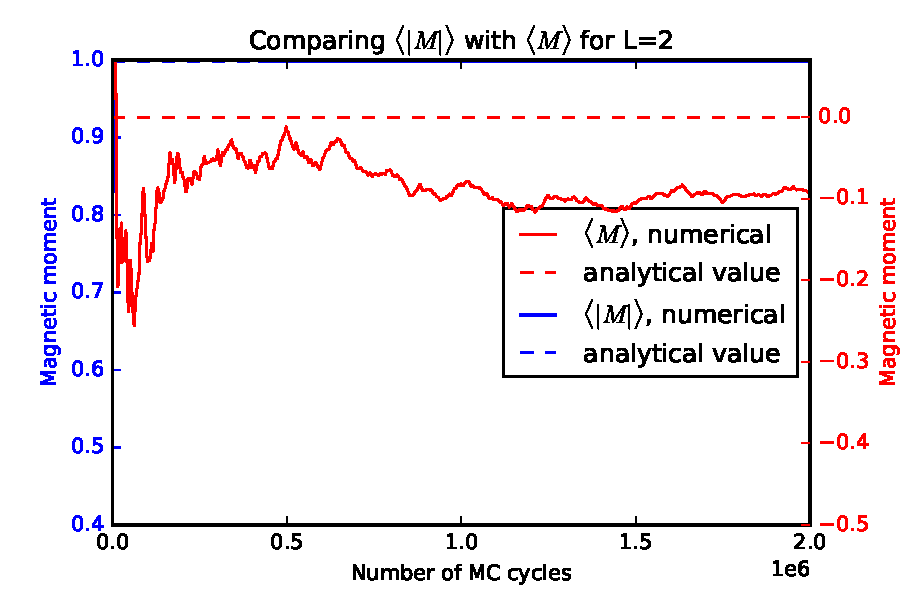
\includegraphics[width=0.7\linewidth]{../results/4b/L_2_mag_magabs}
	\caption{Comparison of the mean magnetization and the mean absolute magnetization. }
	\label{fig:l2magmagabs}
\end{figure}






Due to the smaller fluctuation of  $ \langle \abs{M} \rangle $, the susceptibility for the system was calculated by \begin{equation}
\chi = \frac{1}{k_B T} \left( 	\langle M^2 \rangle - \langle \abs{M}\rangle^2 	\right)\label{eq_X_def_new}
\end{equation}


	\begin{figure}[H]
		\begin{subfigure}[b]{0.49\textwidth}
	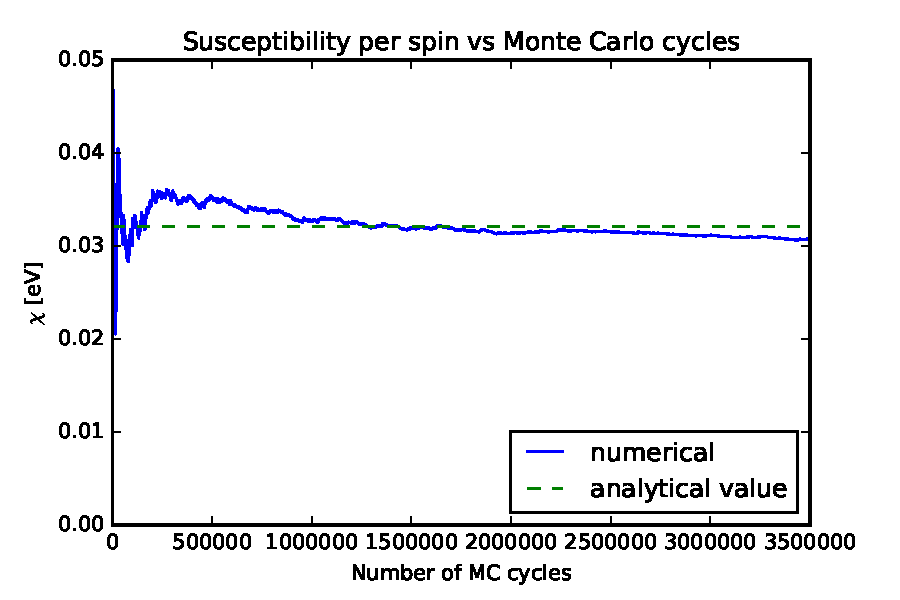
\includegraphics[width=1\linewidth]{../results/4b/L_2_susceptibility}
\caption{}
\label{fig:l2susceptibility}
		\end{subfigure}
		\hfill
		\begin{subfigure}[b]{0.49\textwidth}
		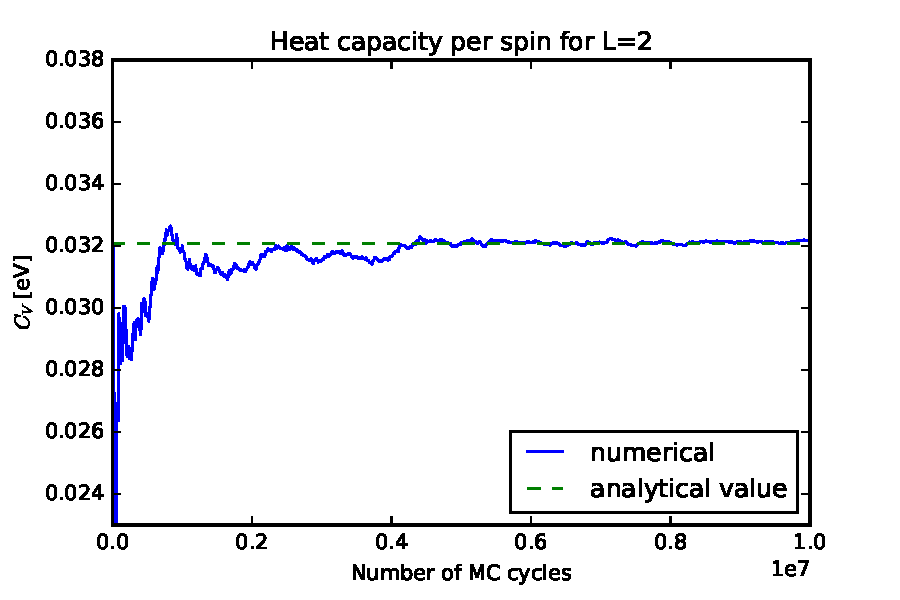
\includegraphics[width=1\linewidth]{../results/4b/L_2_heat_capasity}
\caption{}
\label{fig:l2heatcapasity}
		\end{subfigure}
		\caption{}
	\end{figure}





%\begin{table}[H]
%\caption{This table compares the analytical values for L=2 with the numerical ones after $10^6$ Monte Carlo cycles. The values are in units per spin.}\label{tab:compare_values}
%	\begin{tabular}{ccc}
%		& Numerical: & Analytical:\\ \hline
%		$\left<E\right>$ &   -1.9958 & -1.9960\\
%		$\left<E^2\right>$ &   15.9664 & 15.9679\\
%		$\left<M\right>$ &    0.0451 & 0\\
%		$\left<M^2\right>$ &    3.9930 & 3.9933\\
%		$\left<|M|\right>$ &    0.9986 & 0.9987\\
%		$\chi$ &   3.9849 & 3.9933\\
%		$C_V$& 0.0335 & 0.0321\\
%	\end{tabular}
%\end{table}


\subsection{The L=20 system}


\subsubsection{Initial ordering of the system and equilibrium time}

\begin{figure}[H]
	\begin{subfigure}[b]{0.49\textwidth}
	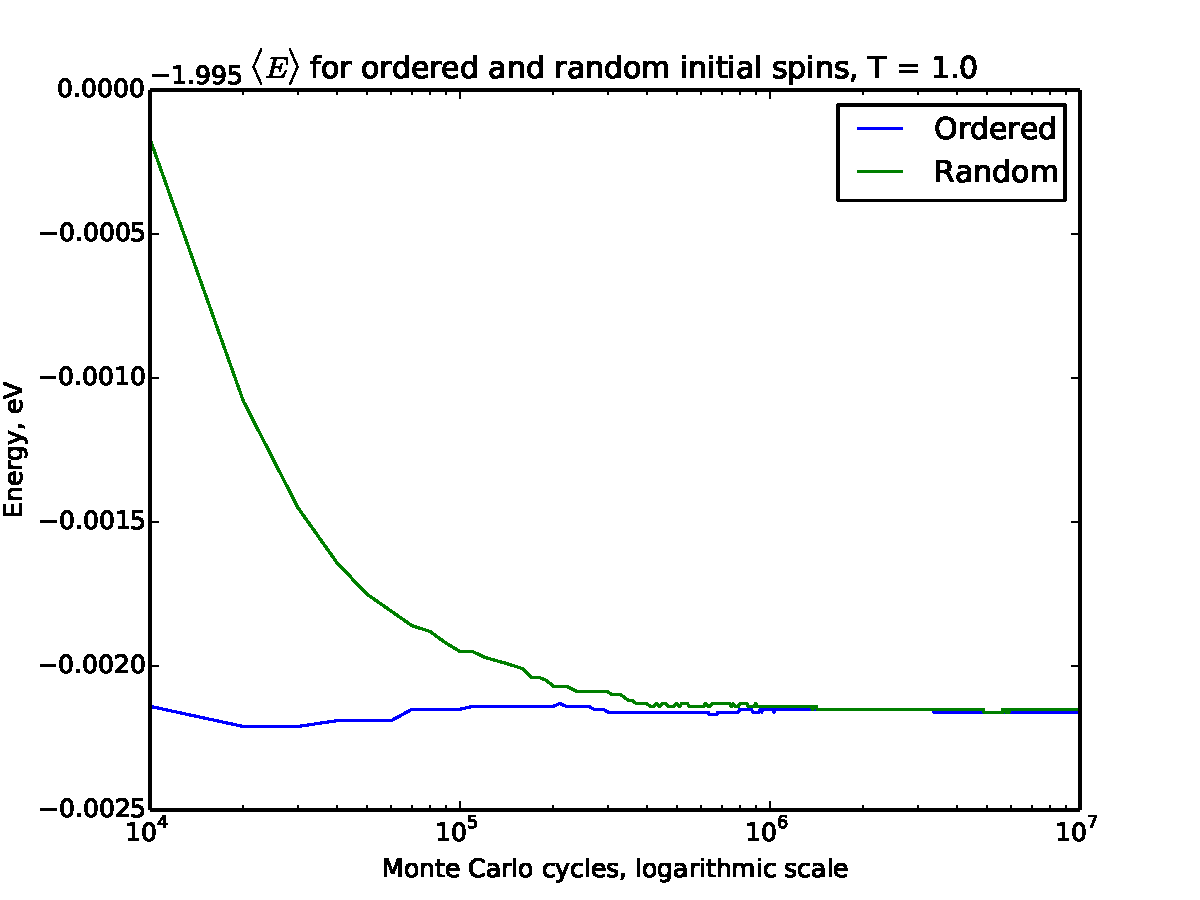
\includegraphics[width=1\linewidth]{../results/4c/ran_order_T1}
\caption{Comparison of the mean energy with both ordered and random initial spin configuration.}
\label{fig:ranordert1}
	\end{subfigure}
	\hfill
	\begin{subfigure}[b]{0.49\textwidth}
	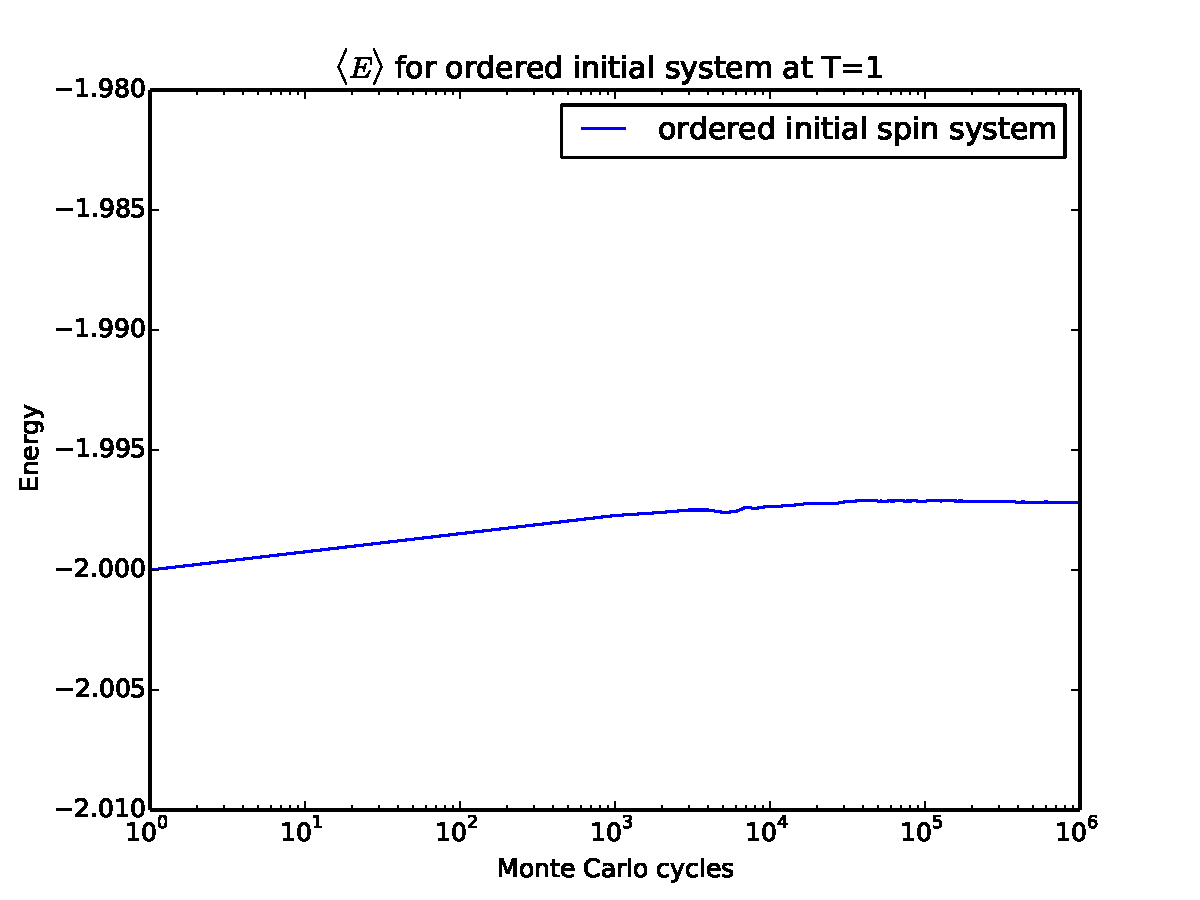
\includegraphics[width=1\linewidth]{../results/4c/order_T1_start}
\caption{Closeup of the $\langle E \rangle $ for the ordered initial configuration}
\label{fig:ordert1start}
	\end{subfigure}
	\caption{Comparison of the mean energy with both ordered and random initial spin configuration at T = 1 $\frac{k_BT}{J}  $ on an logarithmic x axis.}
\end{figure}
Both the initial and the ordered initial matrix converges towards the same value after a significant number of Monte Carlo cycles.  The ordered initial matrix started in the lowest possible energy state. From figure \ref{fig:ranordert1}, the random initial matrix seems to have an equilibration time of approximately $ 10^{5} $ Monte Carlo cycles. As the ordered initial matrix changes a lot less, it is only possible to read this information from figure \ref{fig:ordert1start} and this initial condition also seems to converge after  $ 10^{5} $ Monte Carlo cycles. 

The behaviour in figure \ref{fig:ranordert2} is a bit more chaotic. The equilibrium value of $ \langle E \rangle  $ is higher than for $ T=1 $, and change in value for the first $ 10^{3} $ MC-cycles is large compared to figure \ref{fig:ranordert1}. However, after approximately  $ 10^{5} $ Monte Carlo cycles both the random and ordered initial matrix seems to converge to the same mean energy. In this intervall, between $ 10^{5} $ and $ 10^{6} $ MC-cycles the fluctuations in the mean energy is significantly smaller than between  $ 10^{3} $ and $ 10^{5} $ cycles. 


\begin{figure}[H]
		\centering
	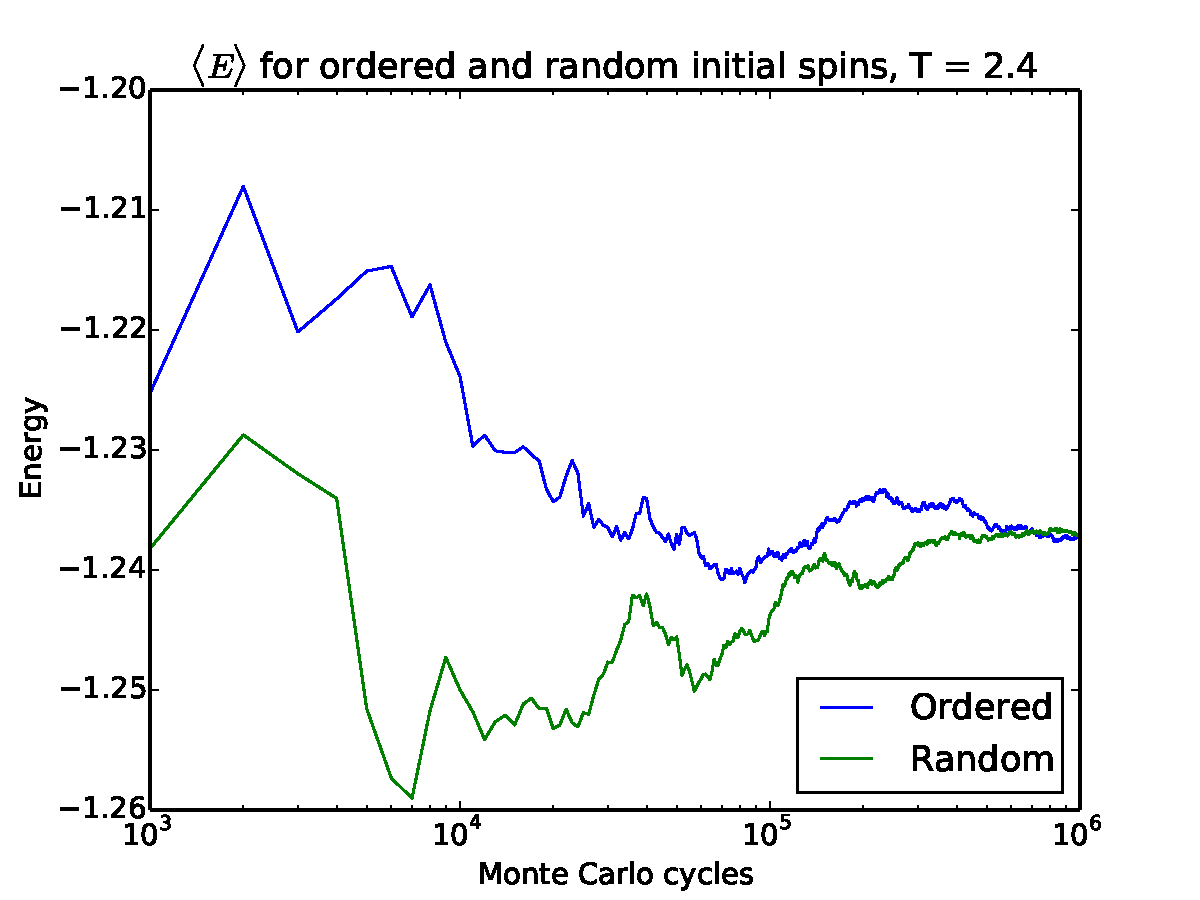
\includegraphics[width=0.7\linewidth]{../results/4c/ran_order_T2}
	\caption{Comparison of the mean energy with both ordered and random initial spin configuration at T = 2.4 $\frac{k_BT}{J}  $ on an logarithmic x-axis.}
	\label{fig:ranordert2}
\end{figure}

Figures \ref{fig:her} provides a closer look at the equilibrium behaviour of the L=20 system. The same trend shown  in figure \ref{fig:ranordert1} and \ref{fig:ranordert2} for the behaviour of the system towards equilibrium is here seen around the equilibrium. For temperature T = 1 the fluctuations are small compared to the fluctuations for T =2.4. In addition the mean magnetization and energy is fully converged around $ 0.4\E{6} $, which is slower than the equilibration time of  $ 0.1\E{6} $ for T =1. Both figures  \ref{fig:L20_mag_T_1} and \ref{fig:L20_mag_T_2-4} show that the energy and magnetization is strongly correlated, converging at the approximately the same time.

	\begin{figure}[H]
	\begin{subfigure}[b]{0.49\textwidth}
		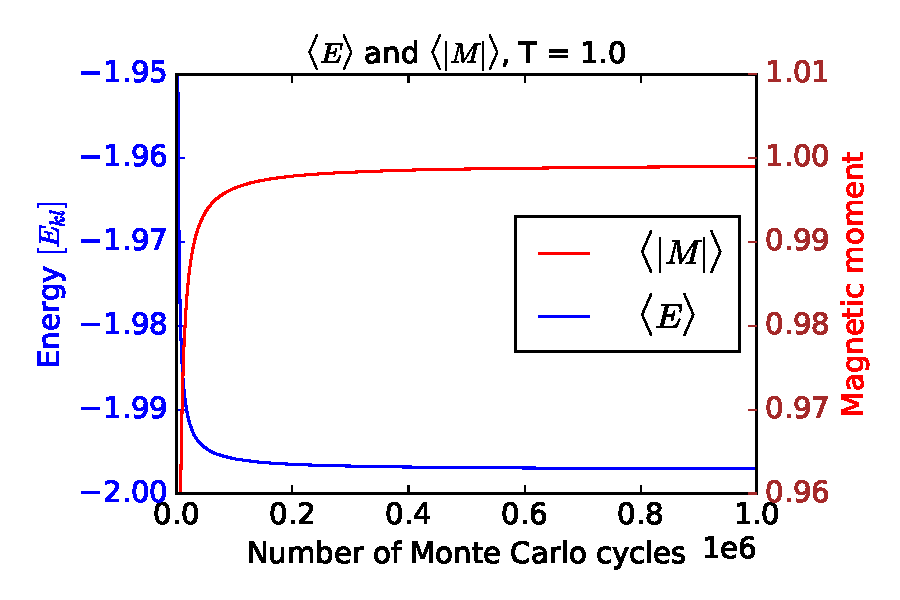
\includegraphics[width=1\linewidth]{../results/4c/En_mag_T1_0}
		\caption{Mean magnetization and energy at T = 1}
		\label{fig:L20_mag_T_1}
	\end{subfigure}
	\hfill
	\begin{subfigure}[b]{0.49\textwidth}
		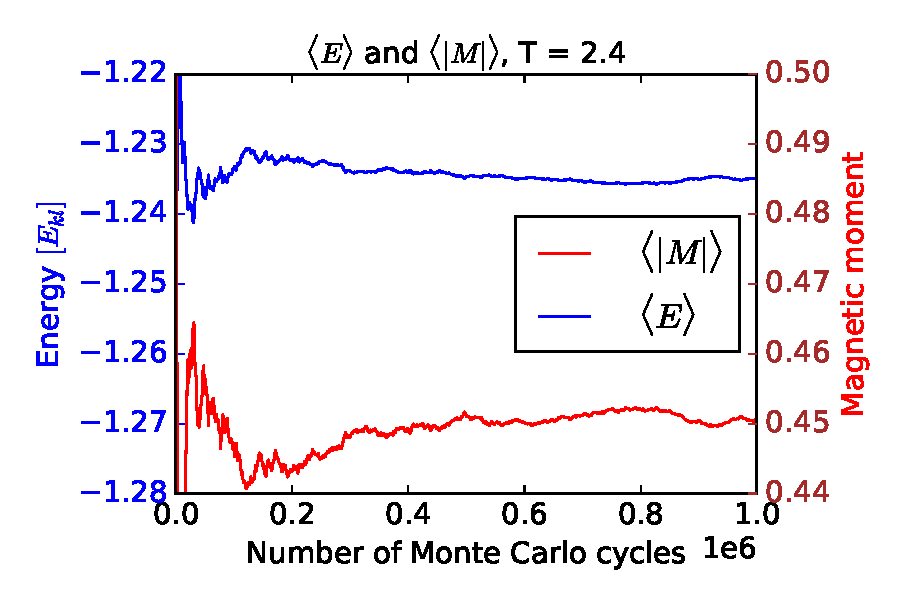
\includegraphics[width=1\linewidth]{../results/4c/En_mag_T2_4}
		\caption{Mean magnetization and energy at T = 2.4}
		\label{fig:L20_mag_T_2-4}
	\end{subfigure}
	\caption{Mean magnetization and energy on a linear x-scale for the randomly initialized  L=20 system at T = 1 and T = 2.4}
	\label{fig:her}
\end{figure}


Figure \ref{fig:l20acceptedconfigs} show how many attempts at changing a spin in the matrix is accepted at equilibrium. Both temperatures show a that fewer than $0.5\%  $ is accepted. Figure \ref{fig:l20acceptedconfigs} shows the total accepted configurations, with the temperature $ T =2.4$ having accepted more configurations. Even though the probability of accepting a change of spin is low, both temperatures accumulate more configurations. However, the gradient of increase is highest between around $ 0\E{6} $, meaning the range $ 0 -10^{5} $ Monte Carlo cycles.

	\begin{figure}[H]
	\begin{subfigure}[b]{0.49\textwidth}
	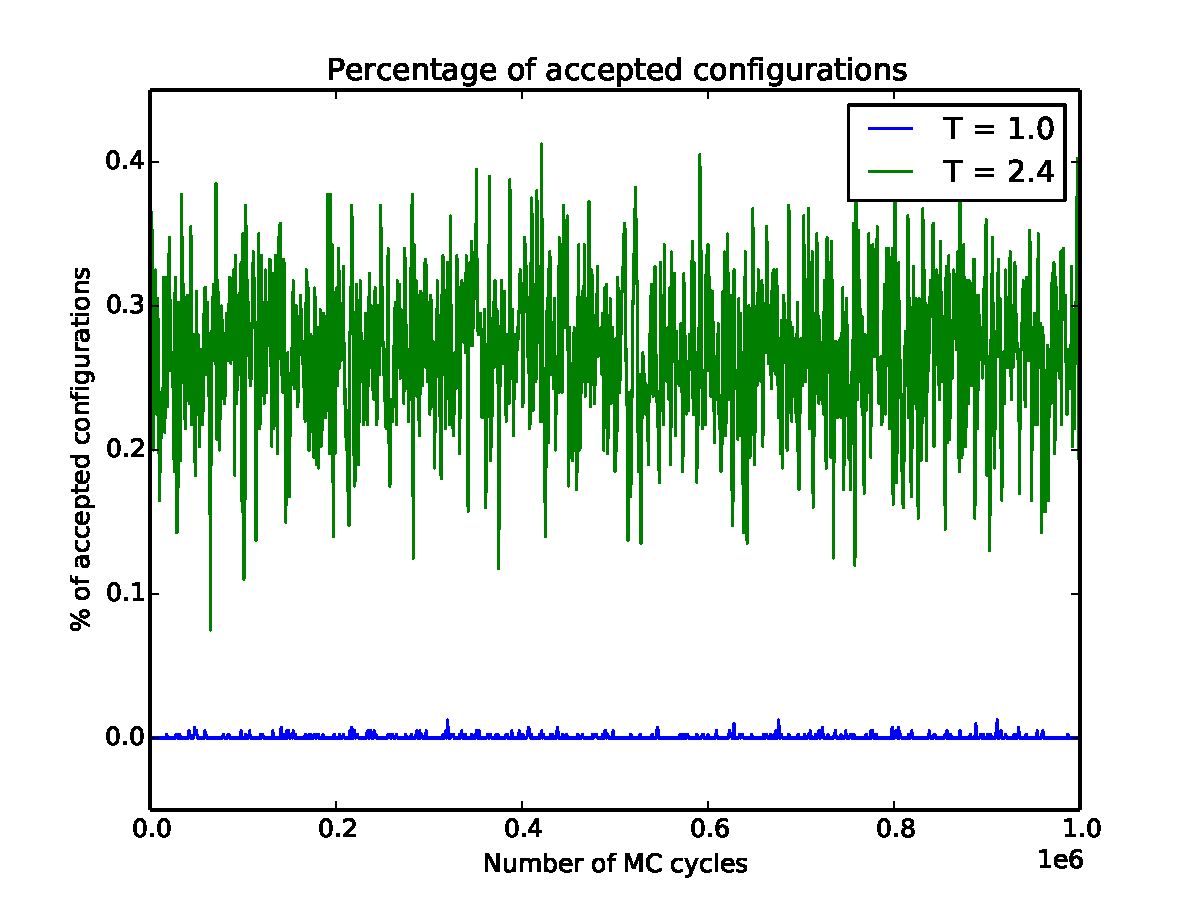
\includegraphics[width=1\linewidth]{../results/4c/L_20_accepted_configs}
\caption{}
\label{fig:l20acceptedconfigs}
	\end{subfigure}
	\hfill
	\begin{subfigure}[b]{0.49\textwidth}
	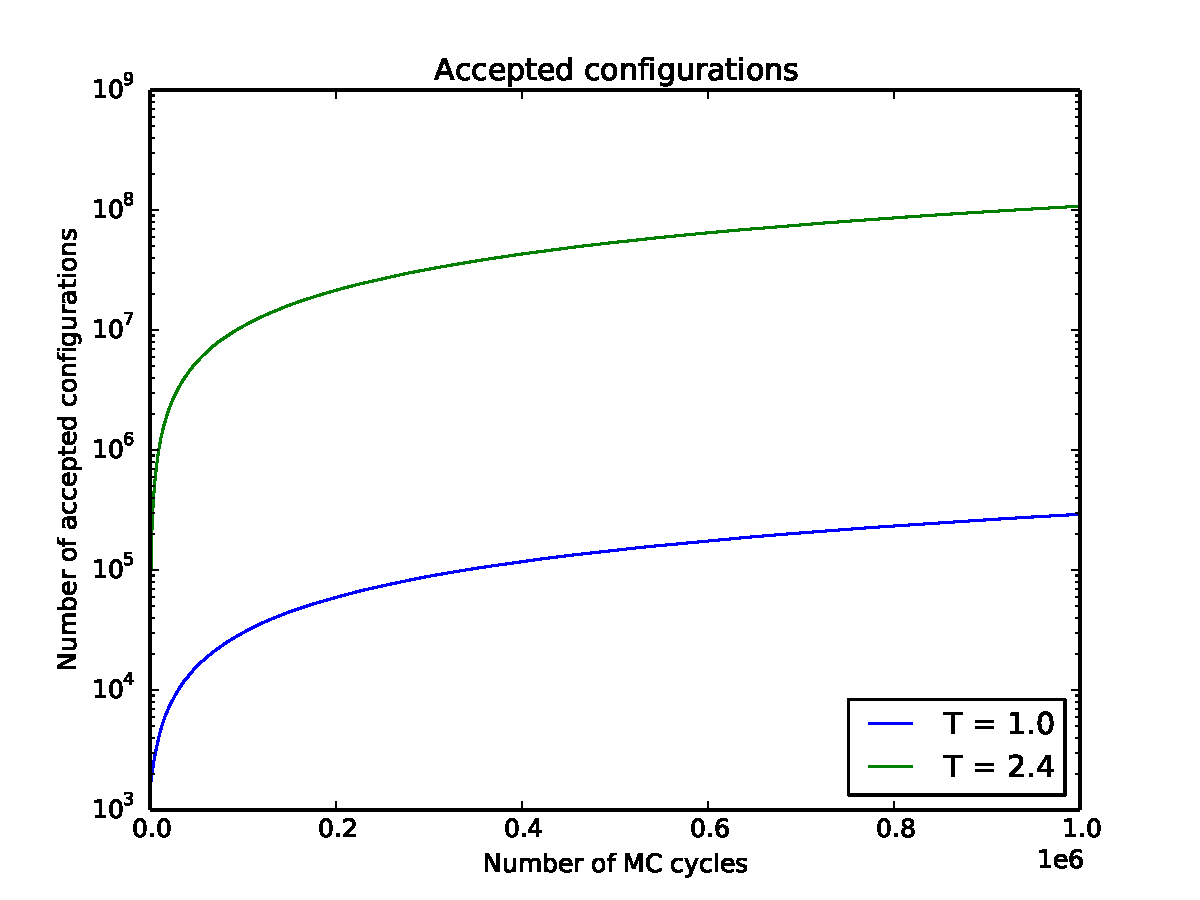
\includegraphics[width=1\linewidth]{../results/4c/L_20_accepted_configs_}
\caption{}
\label{fig:l20acceptedconfigs}
	\end{subfigure}
	\caption{}
\end{figure}











\subsubsection{Probability distrubition  for the L=20 system}


	\begin{figure}[H]
	\begin{subfigure}[b]{0.49\textwidth}
	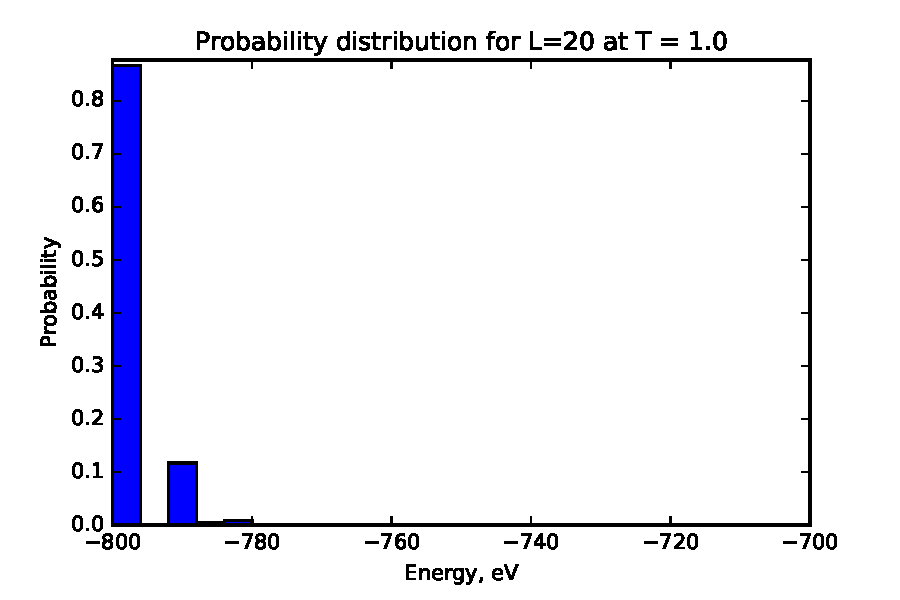
\includegraphics[width=1\linewidth]{../results/4d/PD_T_1MC_1e6}
\caption{Distribution of  energies after equilibrium for T = 1}
\label{fig:pdt1}
	\end{subfigure}
	\hfill
	\begin{subfigure}[b]{0.49\textwidth}
		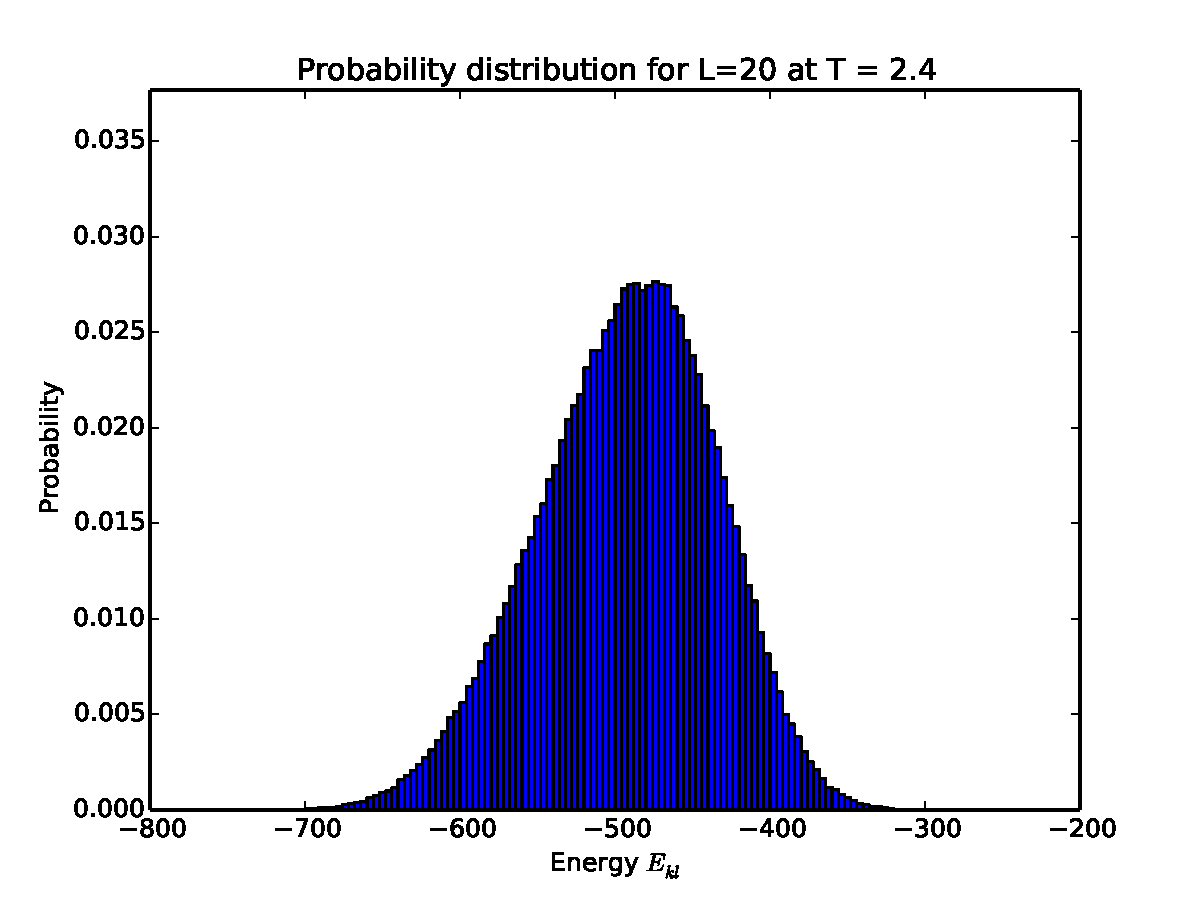
\includegraphics[width=1\linewidth]{../results/4d/PD_T_2MC_1e6}
	\caption{Distribution of  energies after equilibrium for T = 2.4}
	\label{fig:pdt2_4}
	\end{subfigure}
	\caption{Normalized distribution of  energies at equilibrium,  after the $ 5\E{5} $ MC-cycles}
	\label{fig:distribution}
\end{figure}



 Figure \ref{fig:pdt2_4} shows a distribution not unlike a Gaussian distribution, while  \ref{fig:pdt1} has a high probability for the lowest energies and a probability that goes towards zero for higher energies. This is coherent with the data in table \ref{tab:varians}, where the higher temperature $ T = 2.4 $ has both significantly higher standard deviation and variance than the $ T = 1 $ case. 

\begin{table}[H]\caption{Table of the standard deviation and expectation value of energy for the L = 20 system} \label{tab:varians}
	\begin{tabular}{ccc}
		Temperature ($ \frac{k_BT}{J} $)& $ \sigma_E^2 $&$ \sigma_E$ \\\hline
		2.4 &3213.71 & 56.69\\
				1 &11.36  & 3.37 
	\end{tabular}
\end{table}



\subsection{Phase transition and Critical temperature}

In figures \ref{fig:4ecv} and \ref{fig:4ex}, both the susceptibility and heat capacity peaks around  a temperature of 2.3  for all grid sizes. The critical temperatures is stated in table \ref{tab: T_C}. Around the critical temperature, the interval between the temperatures is $ dT = 0.01 $, while between $ T = 2.1\rightarrow2.2 $ and $ T = 2.4\rightarrow2.6  $ it is approximately $ dT = 0.05 $. 

\begin{figure}[H]
	\centering
	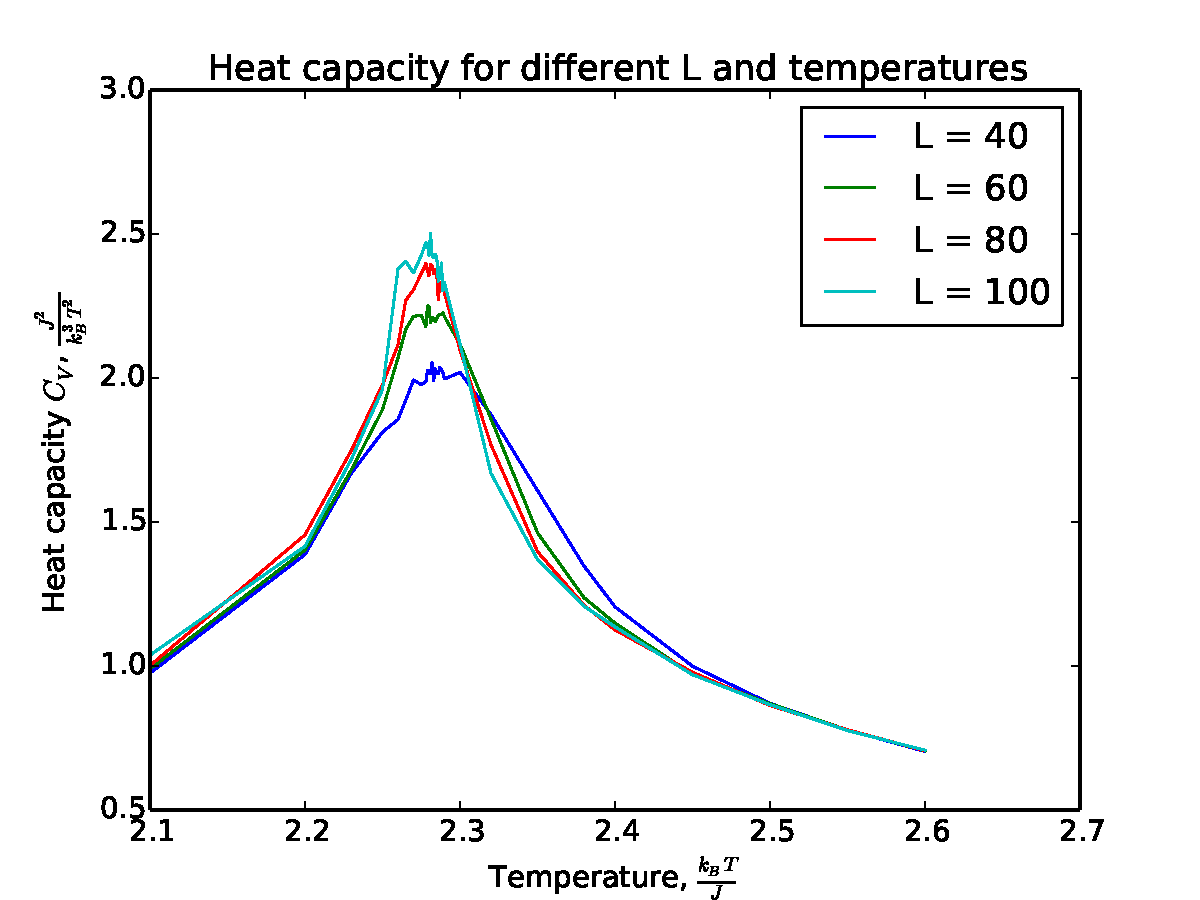
\includegraphics[width=0.7\linewidth]{../results/4e/4e_Cv}
	\caption{Susceptibility as a function of temperature and matrix size}
	\label{fig:4ecv}
\end{figure}

\begin{figure}[H]
	\centering
	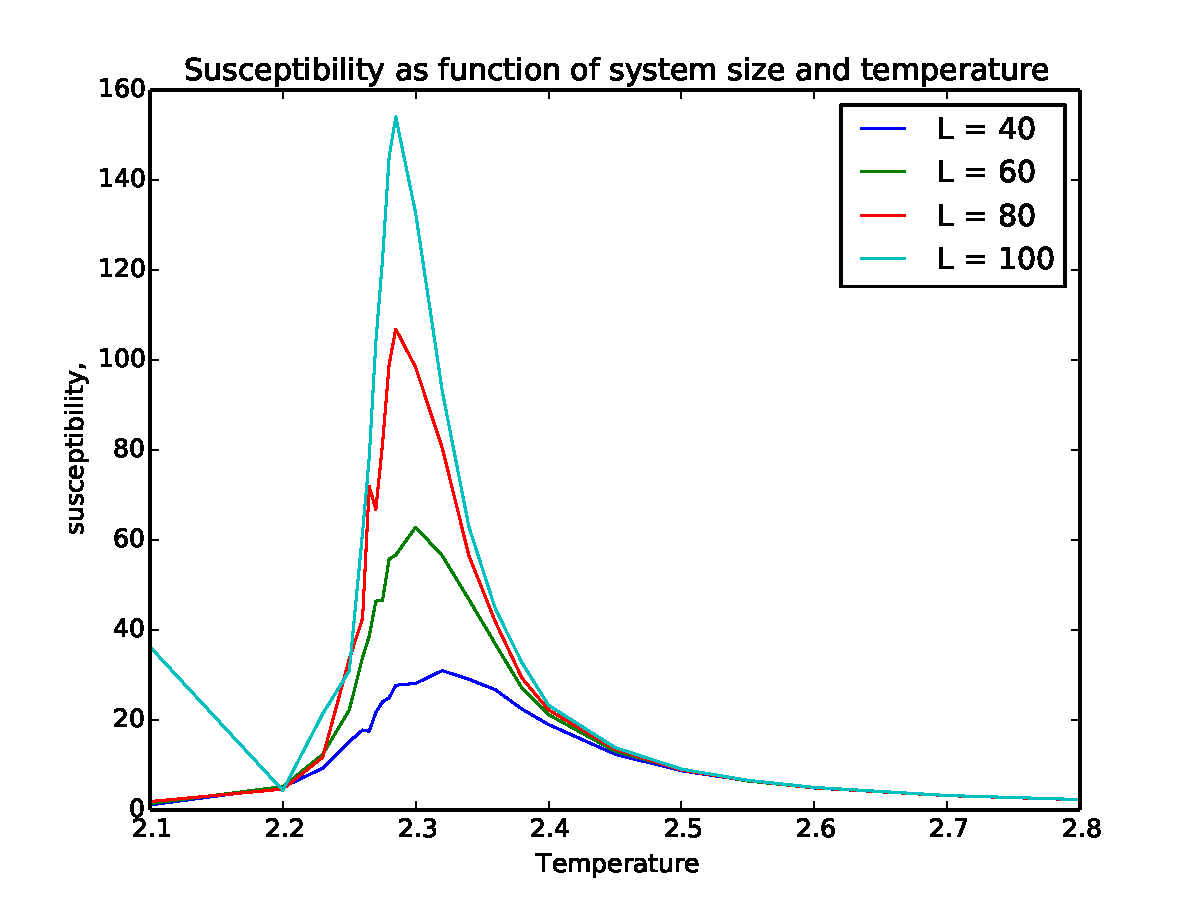
\includegraphics[width=0.7\linewidth]{../results/4e/4e_x}
	\caption{Heat capacity as a function of temperature and matrix size}
	\label{fig:4ex}
\end{figure}

At the critical temperature, the energies of the different systems is no longer the same, see figure \ref{fig:4eenergy}. But they are following the same trend, increasing mean energy as the temperature increases. However, the magnetization drops suddenly towards a $ \langle M \rangle  =0$ at the critical temperature. The trend is also that larger lattices goes faster towards $ \langle M \rangle  =0$ than the smaller lattices.

	\begin{figure}[H]
	\begin{subfigure}[b]{0.5\textwidth}
	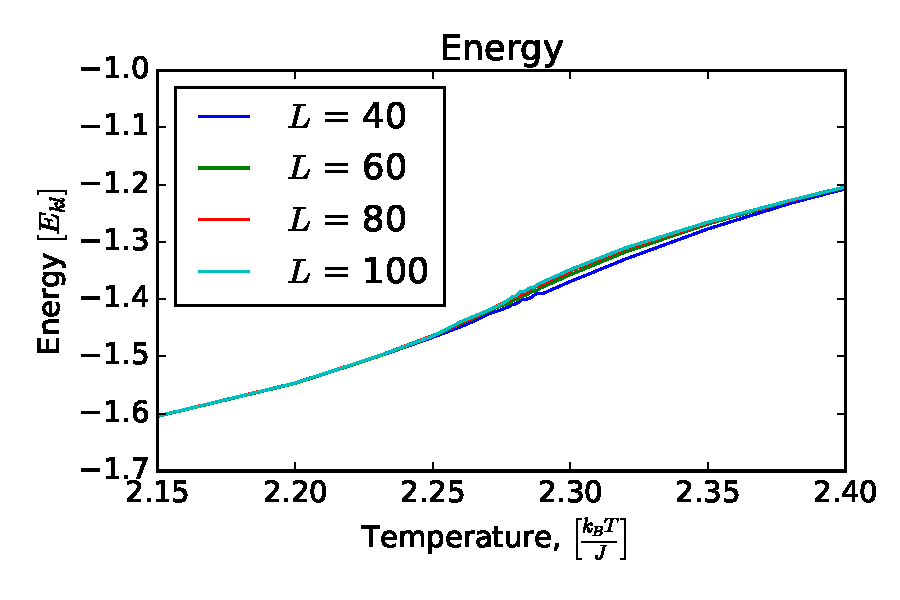
\includegraphics[width=1\linewidth]{../results/4e/4e_energy}
\caption{Mean energy as a function of temperature and matrix size}
\label{fig:4eenergy}
	\end{subfigure}
	\hfill
	\begin{subfigure}[b]{0.5\textwidth}
	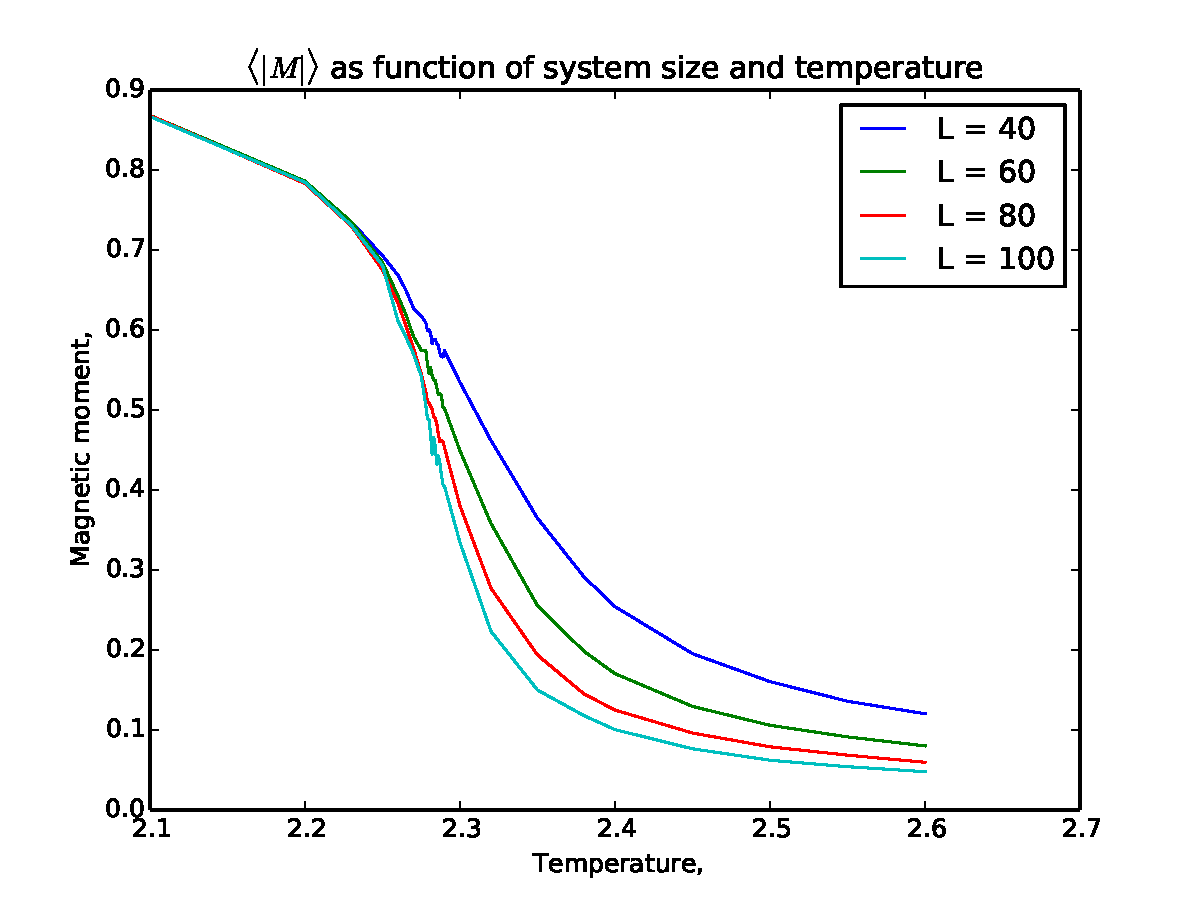
\includegraphics[width=1\linewidth]{../results/4e/4e_mag}
\caption{Mean magnetization as a function of temperature and matrix size}
\label{fig:4emag}
	\end{subfigure}
	\caption{Mean magnetization and energy as a function of temperature and matrix size}
\end{figure}

For the critical temperatures there is no clear trend, see table \ref{tab: T_C}. In order to find $ T_C $ for a system with $ L=\infty $, the data from table \ref{tab: T_C} was plotted against the inverse lattice size. This gave a $ T_C(L = \infty) =T_C(1/L = 0) \simeq 2.2777  \frac{k_BT}{J}  $. 

\begin{table}[H]
	\caption{text}
	\label{tab: T_C}
	\begin{tabular}{cccccc}
		 L & $T_C$ \\ \hline    
     40 & 2.282 \\ 
 60 & 2.279 \\ 
 80 & 2.278 \\ 
 100 & 2.281 \\ 

	\end{tabular}
\end{table}


\begin{figure}[H]
	\centering
	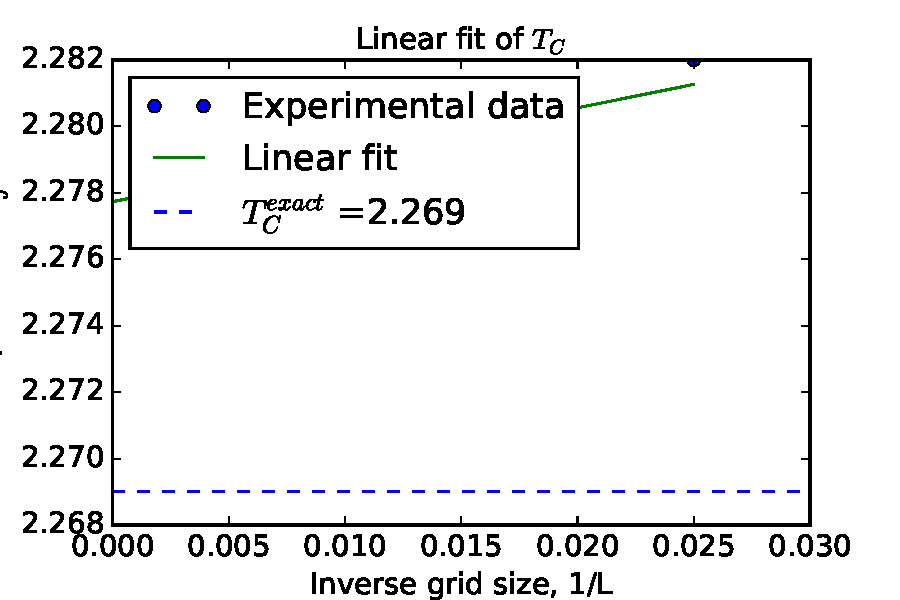
\includegraphics[width=0.7\linewidth]{../results/4e/linfit}
	\caption{linear fit of the critical temperatures as a function of inverse grid size}
	\label{fig:linfit}
\end{figure}




\subsection{Speedup}
From table \ref{tab:speedy} it is clear that computing in parallel gives a speedup. The calculations were carried out for  the case of $ L=60 $, two temperatures and a total of $ 10^6 $ MC cycles on a computer with a 2 core i5 processor. This yields a speedup of $ \frac{T_1}{T_2} = 0.598  $

\begin{table}[H]\caption{Overview of the time spent computing the L=60 system with two temperatures.} \label{tab:speedy}
	\begin{tabular}{cc}
		Number of cores:& CPU time [s]: \\ \hline
		1 & 513.069\\
		2 & 306.975\\
	\end{tabular}
\end{table}
